La classe de l'Èlia ha dissenyat el logotip següent per a pintar-lo a la paret de l'institut:
\begin{center}
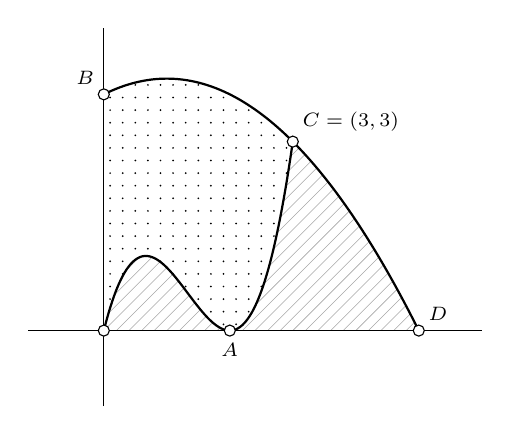
\begin{tikzpicture}[x=0.8cm,y=0.8cm]
  \begin{scope}
    \clip (0,0) -- plot[domain=0:3,samples=60,smooth] (\x,{(\x)^3-4*(\x)^2+4*(\x)})
      -- plot[domain=3:5,samples=40,smooth] (\x,{4-((\x)-1)^2/4}) -- cycle;
    \foreach \t in {-5,-4.8,...,5} \draw[gray!70,very thin] (\t,0) -- ++(4,4);
  \end{scope}
  \begin{scope}
    \clip plot[domain=0:3,samples=60,smooth] (\x,{4-((\x)-1)^2/4})
      -- plot[domain=3:0,samples=60,smooth] (\x,{(\x)^3-4*(\x)^2+4*(\x)}) -- cycle;
    \foreach \i in {0.1,0.3,...,3} \foreach \j in {0.1,0.3,...,4} \fill (\i,\j) circle (0.35pt);
  \end{scope}
  \draw (-1.2,0) -- (6,0);
  \draw (0,-1.2) -- (0,4.8);
  \draw[\colorgrafica,thick] plot[domain=0:3,samples=80,smooth] (\x,{(\x)^3-4*(\x)^2+4*(\x)});
  \draw[\colorgrafica,thick] plot[domain=0:5,samples=80,smooth] (\x,{4-((\x)-1)^2/4});
  \foreach \p in {(0,3.75),(3,3),(2,0),(5,0),(0,0)} \draw[fill=white] \p circle (2pt);
  \node[above left,font=\scriptsize] at (0,3.75) {$B$};
  \node[above right,font=\scriptsize] at (3,3) {$C=(3,3)$};
  \node[below,font=\scriptsize] at (2,-0.05) {$A$};
  \node[above right,font=\scriptsize] at (5,0) {$D$};
\end{tikzpicture}
\end{center}
La corba que passa pel punt $A$ és $y=f(x)$, amb $f(x)=x^3-4x^2+4x$, i la que passa pels punts $B$, $C=(3,3)$
i $D$ és $y=g(x)$, amb $g(x)=-\left(\dfrac{x-1}{2}\right)^2+4$.

\begin{apartats}

\apartat{0,75}
Calculeu les coordenades dels punts $A$, $B$ i $D$.

\begin{solucio}
El punt $A$ és un punt de tall de $y=f(x)$ amb l'eix $OX$: $x^3-4x^2+4x=0\rightarrow x(x-2)^2=0\rightarrow
x=0,\ x=2$. Per tant, el punt $A$ té per coordenades $A=(2,0)$. El punt $D$ és un punt de tall de $y=g(x)$ amb
l'eix $OX$:
\[
-\left(\frac{x-1}{2}\right)^2+4=0\;\rightarrow\;x^2-2x-15=0\;\rightarrow\;x=\frac{2\pm\sqrt{4-4(-15)}}{2}=-3,\ 5 .
\]
Descartem la solució negativa i podem afirmar, per tant, que el punt $D$ té coordenades $D=(5,0)$.
Finalment, el punt $B$ és el punt de tall de $y=g(x)$ amb l'eix $OY$; com que
$g(0)=-\left(\frac{0-1}{2}\right)^2+4=\frac{15}{4}$, es tracta del punt $B=\left(0,\frac{15}{4}\right)$. Les
coordenades del punt $C$ ja ens les dona l'enunciat, $C=(3,f(3))=(3,g(3))=(3,3)$.

\textit{Pauta oficial:} 0,25 pel càlcul de cadascun dels tres punts demanats.
\end{solucio}

\apartat{1,25}
Calculeu l'àrea de la zona puntejada.

\begin{solucio}
La zona puntejada és l'àrea compresa entre $g(x)$ i $f(x)$ des de $x=0$ fins a $x=3$:
\begin{align*}
A_1&=\int_0^3\left(-\left(\frac{x-1}{2}\right)^2+4-\left(x^3-4x^2+4x\right)\right)dx
=\int_0^3\frac{-4x^3+15x^2-14x+15}{4}\,dx\\
&=\frac14\left[-x^4+5x^3-7x^2+15x\right]_0^3=9\ \text{u}^2 .
\end{align*}

\textit{Pauta oficial:} 0,5 pel plantejament de l'àrea de la zona puntejada (amb els límits d'integració
correctament col·locats), 0,5 per la primitiva i 0,25 pel càlcul final.
\end{solucio}

\apartat{0,5}
Els alumnes volen pintar la part puntejada de color blau i la part ratllada de color vermell. Sabent que l'àrea
total del logotip és $\dfrac{175}{12}\ \text{m}^2$, de quin color necessitaran més pintura?

\begin{solucio}
Sabent que l'àrea total del logotip és de $\frac{175}{12}=14{,}583\ldots\ \text{u}^2$, la zona ratllada tindrà
una àrea de $14{,}583\ldots-9=5{,}583\ldots\ \text{u}^2$. Per tant, per pintar el logotip de la manera que
volen, els caldrà més pintura blava que vermella.

\textit{Pauta oficial:} 0,5 per la resposta correcta.
\end{solucio}

\end{apartats}
